\begin{problem}{\textbf{\textsc{Electric Slide}}} 
Consider a gas of small particles, each with charge $q$, inside an origin-centered spherical chamber of radius $R$. A uniform electric field $E\hat{\mathbf{x}}$ is applied inside the chamber. The field is adjusted until point $(R,0,0)$ has pressure $P_0$ and point $(-R,0,0)$ has pressure $P_0/2$ (at equilibrium). 

The electric field is quickly decreased to zero, and the gas comes to equilibrium again. If the final pressure in the chamber is $P_1$, find $P_1/P_0$. Neglect interactions between particles and assume that the temperature of the gas remains nearly constant.
\vspace{-0.5cm}
\begin{center}
    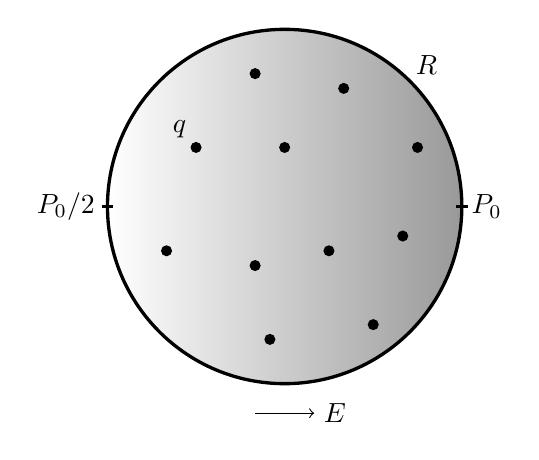
\begin{tikzpicture}[scale = 0.75, dot/.style = {circle, fill, minimum size=#1, inner sep=0pt, outer sep=0pt}]
    \draw[very thick,left color=white, right color = white!60!black] (0, 0) circle (3);
    \draw[very thick] (2.9,0)--(3.1,0);
    \node at (3, 0) [right]{$P_0$};
    \draw[very thick] (-3.1,0)--(-2.9,0);
    \node at (-3.05,0) [left]{$P_0/2$};
    \node at (2,-0.5) [dot=4]{};
    \node at (-0.5, -1) [dot=4]{};
    \node at (1, 2) [dot=4]{};
    \node at (0, 1)[dot=4]{};
    \node at (0.75, -0.75)[dot=4]{};
    \node at (-2, -0.75)[dot=4]{};
    \node at (-1.5, 1) [dot=4]{};
    \node at (1.5, -2) [dot=4]{};
    \node at (-0.5, 2.25) [dot=4]{};
    \node at (-0.25, -2.25) [dot=4]{};
    \node at (2.25, 1) [dot=4]{};
    \node at (-1.5, 1) [above left]{$q$};
    \node at (2.4, 2.4) {$R$};
    \draw [->] (-0.5, -3.5) -- (0.5, -3.5) node[right]{$E$};
    \end{tikzpicture}
\end{center}
\end{problem}
